\documentclass[12pt]{ltjsarticle}
\usepackage{semi}

\begin{document}
\begin{titlepage}
  \begin{center}
  
    \vspace*{20truept}
    
    {\LARGE 2023年度 卒業論文} 
    
    \vspace*{75truept}
    
    {\Huge } %論文タイトル

    \vspace{10truept}

    {\Huge 民俗芸能継承問題における\\小学生向け学習教材の開発} %論文タイトル 長い場合 改行1

    \vspace{10truept}

    {\Huge } %論文タイトル 改行2

    \vspace{85truept}
    
    {\LARGE 指導教員 須田 宇宙 准教授}
    
    \vspace{60truept}
    
    {\LARGE 千葉工業大学 情報ネットワーク学科}
    
    \vspace{15truept}
    
    {\LARGE 須田研究室}
    
    \vspace{70truept}
    
    {\LARGE 1932102 氏名 永塚 迅一 } % 氏名は消さない 学生番号 氏名 名前

    \vspace{70truept}
    
  \end{center}
  \begin{flushright}

    {\LARGE 提出日 2023年1月17日}
  
  \end{flushright}
\end{titlepage}







\tableofcontents
\newpage
\section{緒言}

%背景

日本には今もなお,人々を魅了し感動を与える伝統芸能がある.伝統芸能は,日本舞踊,演劇,演芸,歌,音曲,工芸,芸道の7種類に分けられ,さらにそこから細かく分かれていく.しかし,高齢化や後継者不足により満足に活動することができない問題がある.

茨城県の伝統芸能に「女沼のささら」という獅子舞があり,ささら保存会によって保存継承がなされている.また、地元小学校の運動会では図\ref{fig:運動会}のように児童がささらを踊り,観客を楽しませる.
\begin{figure}[h]
\begin{center}
 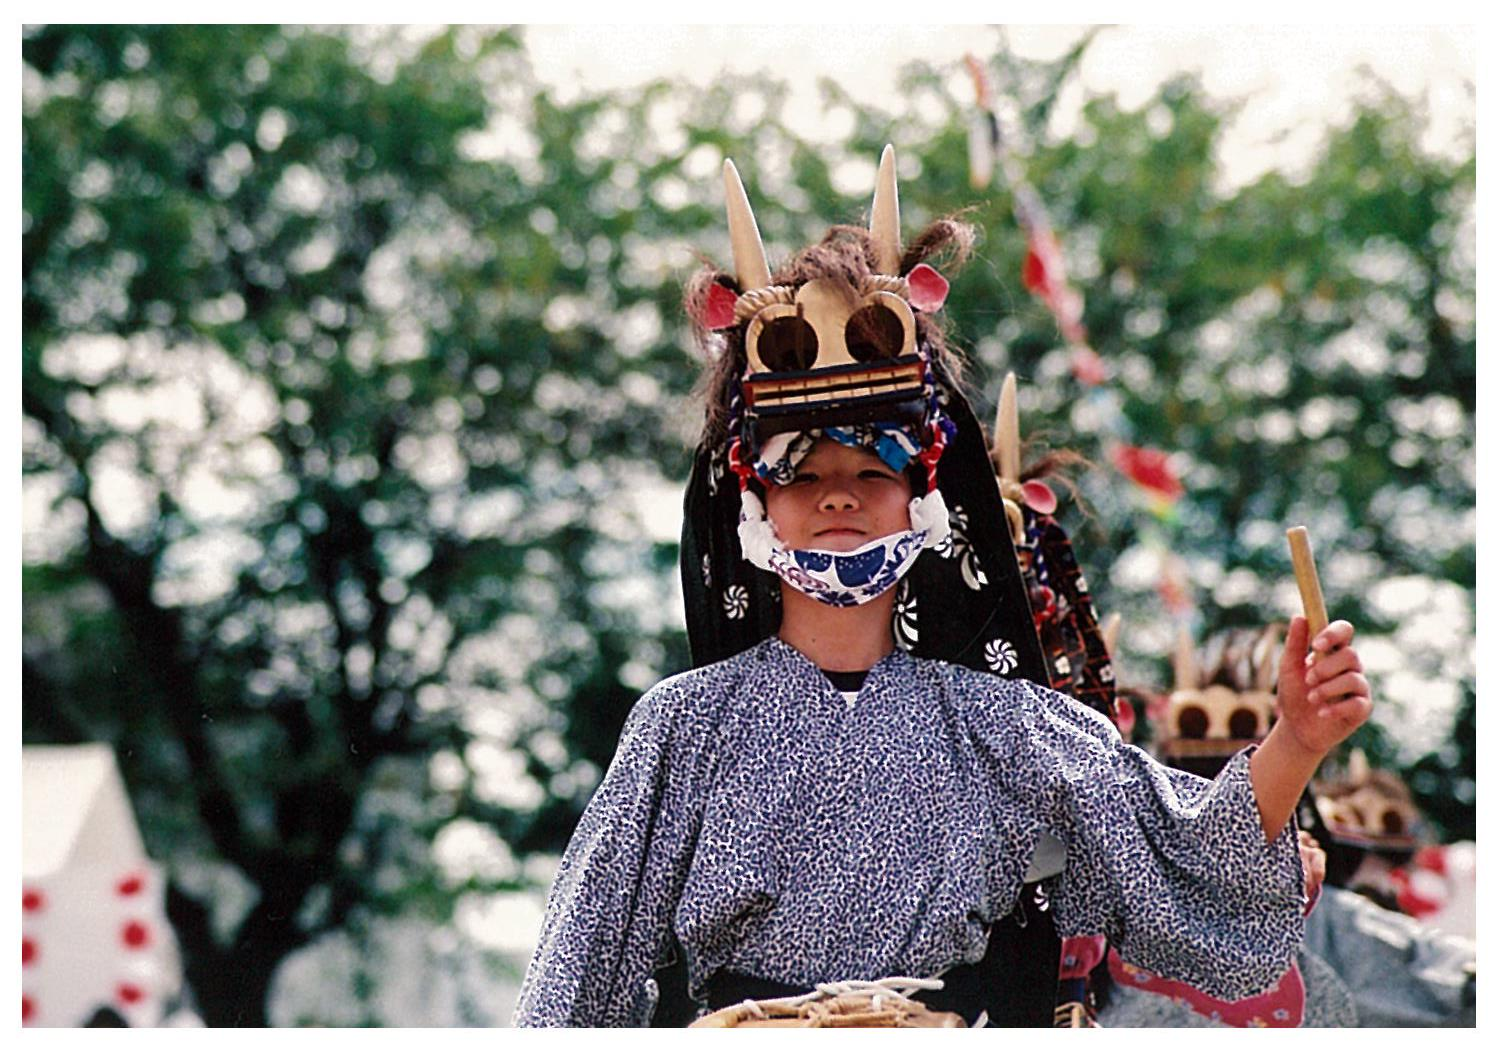
\includegraphics[clip,width=85mm]{undoukai2.jpg}
\end{center}
 \caption{運動会でのささら発表の様子}
 \label{fig:運動会}
\end{figure}


%問題点
小学校の運動会で披露するささらは,4年生から6年生の選抜された代表児童を中心に全員参加で踊る.そこでささら保存会が運動会前に,代表児童に数回指導を行うのだが,ささら保存会の人数は年々減ってきており,代表児童に対して十分な指導ができないという問題点がある.

%目的
そこで本研究では,ささらの踊りを学習できる教材を開発し,ささら保存会の教えと併用することで代表児童に十分な指導を可能にすることを目的とする.

\newpage
\section{日本の伝統芸能について}

\subsection{概要}
日本における伝統芸能とは古くから人々によって伝承され,修行や稽古を重ねて身に着けた技術や芸術の事をいう.伝統芸能の多くは,西洋文化の影響を受ける前から日本にある文化を指し,明治時代以前に大成したもである.そもそも芸能とは,四季の風物を活かして,祭りや豊作に感謝をすると同時に,唄や儀式を通して神様へ捧げるものであった.そのため,当時は芸能が全国各地で行われていたため,踊りや歌にその土地の独自性が加わり,数多くの芸能が誕生した.それが時を経て,現在も人々を魅了し続けているのである.

伝統芸能という括りの中に民俗芸能がある.民俗芸能とは,それぞれの地域の特色が強く入った伝統芸能であり,強い独自性がある。本研究では,民俗芸能を伝統芸能の一部と認識する.

\subsection{伝統芸能の種類}
伝統芸能は,大きく分けて日本舞踊,演劇,演芸,唄,音曲,工芸の7種類に分類される.さらにそこから細かく分類される.
\subsubsection{日本舞踊}
日本舞踊は,踊り,舞,振りの3つの要素を持つ日本の伝統的な踊りである.踊る際は,音楽に合わせて,登場人物の心情を表現する.

日本舞踊には,神楽,田楽,雅楽,舞楽,猿楽,白拍子,延年,曲舞,上方舞,大国舞,恵比寿舞,纏舞,念仏踊り,盆踊り,歌舞伎舞踊の15種類の伝統芸能がある.
\subsubsection{演劇}
演劇は,観客を前に体全体を使って仕草や身振りをし,物語や人物の心情を演じて見せる芸術である.

演劇は,能楽,歌舞伎,人形浄瑠璃の3種類の伝統芸能がある.能楽に関しては,さらに能,狂言の2つに分けられる.
\subsubsection{演芸}
演芸は,観客を前に演じる芸能で,演劇とはことなり,1人や少人数で演じる芸能である.

演芸には,講談,落語,浪花節,奇術,萬歳,俄,梯子乗り,女道楽,太神楽,かみきり,曲独楽,写し絵,花火の13種類の伝統芸能がある.
\subsubsection{歌}
歌は,言葉を用いて,人の心情や外の景色,季節感などを表現する芸能である.

歌は,和歌,俳諧,琉歌の大きく3種類に分けられる.
\subsubsection{音曲}
音曲は,楽器や人の声を使い披露される伝統芸能である.1人で演じることが多く,達者な喋りと三味線で観客を魅了する.

音曲は,雅楽,邦楽,浄瑠璃節,唄の4種類に分けられる.

\subsubsection{工芸}
工芸は,古くから先祖代々継承してきた技術で,工業製品を作る芸能である.

工芸は,彫金,漆器,陶芸,織物の4種類に分けられる.

\subsubsection{芸道}
芸道は,継承される技術だけでなく,宗教や哲学的背景,身分制度などの思想が反映された技芸である.

芸道は,茶道,華道,武道,書道,華道の5種類に分けられる.



\newpage
\subsection{伝統芸能の問題点}
日本独自の文化であり,先祖代々に技術や技芸を受け継がれてきた伝統芸能であるが,現在では高齢化と後継者不足の問題がある.

伝統芸能の主要な歌舞伎では,芸を代々継承している家元だけでは後継者が足りず,日本芸術文化振興会は一般から人を集め育成を行っている.
しかし,近年は一般からの志願者数が少なく,歌舞伎俳優は2019年度以降5人以下と低迷している.

伝統工芸では,需要が減少しており,従業員を雇用するのが難しい現状がある.総務省行政評価局の伝統工芸の地域資源としての活用に関する
実態調査では,伝統工芸の産地において,「需要の減少」「後継者の不足」「原材料・用具等の不足」を問題視している\cite{sa1}.図\ref{fig:図2}では,直近29年度
までの,経済産業大臣が指定する伝統工芸品データを示している.生産額,従業員数ともに顕著に減少している.

\vskip\baselineskip
\begin{figure}[h]
\begin{center}
 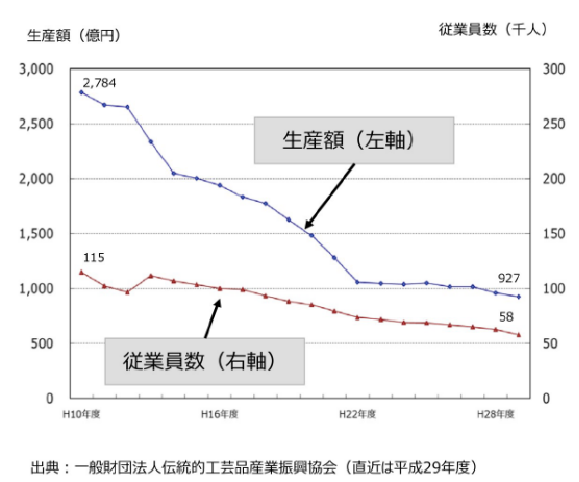
\includegraphics[clip,width=85mm]{figures/dentoukougei.pdf}
\end{center}
 \caption{良い例と悪い例を用いて解説しているページで,十分なおどりの情報を得ることができましたか}
 \label{fig:図2}
\end{figure}

地域においても,問題がある.岩手県の北上市は100を超える民俗団体があり,民俗芸能が盛んな市である.北上市は2018年に
北上市民俗芸能団体連合会加盟団体アンケ―トを加盟47団体を対象に実施した\cite{sa2}.その結果,図\ref{fig:図3}では,36団体が後継者不足であった.
また,15団体が指導者の高齢化であり,継続するためには,若手の参入が必須である.
\vskip\baselineskip
\begin{figure}[h]
\begin{center}
 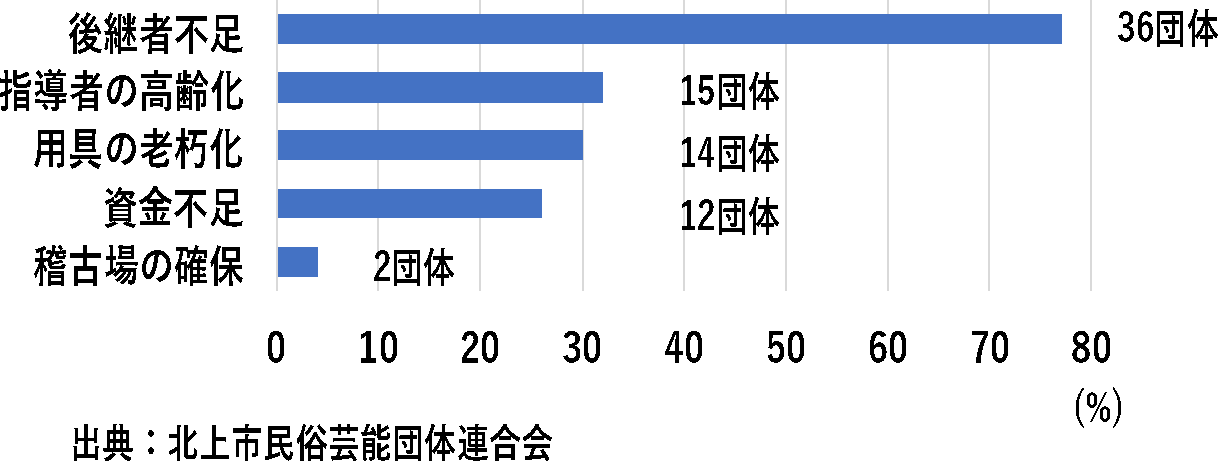
\includegraphics[clip,width=85mm]{figures/kigagami.pdf}
\end{center}
 \caption{各団体の運営におけるなやみ}
 \label{fig:図3}
\end{figure}





上記のように伝統芸能の広い範囲で,後継者が不足しており,現役で活躍している人の高齢化が進んでいる.そのことによって,技を後世に伝えることができず,衰退している.





\newpage
\section{女沼のささら}
\subsection{概要}
女沼のささらは,地元の女沼地区に伝わる民俗芸能の一つである.「前獅子」\footnote{「前獅子」は「太夫獅子」ともいう}「女獅子」「後獅子」の「3人立ち」からなり,
腹には小太鼓を抱き,両手に持ったバチで叩きながら舞う。前,後獅子は紺,女獅子は赤の上着に袴を身に着け,草履をはいている.舞っている様子を図\ref{fig:図4}に示す.
獅子の他には,獅子が舞う際に笛を奏でている笛担当が数名いる.
\vskip\baselineskip
\begin{figure}[h]
\begin{center}
 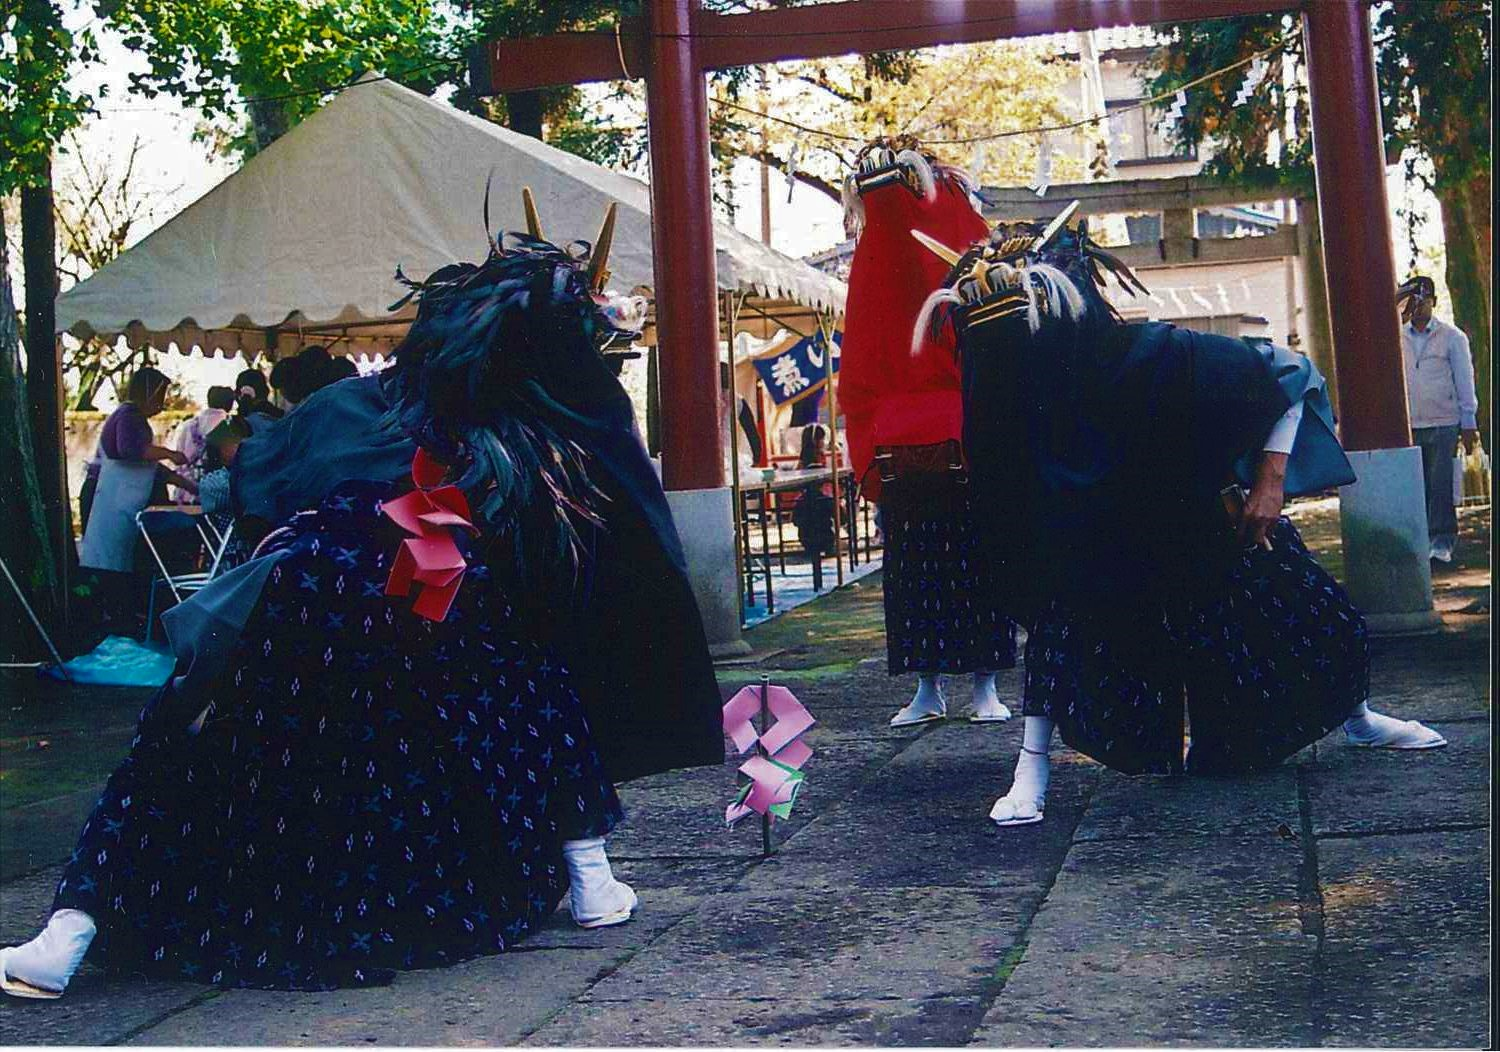
\includegraphics[clip,width=85mm]{figures/mai.jpg}
\end{center}
 \caption{ささら舞の様子 左側が後獅子 中央が女獅子 右側が前獅子}
 \label{fig:図4}
\end{figure}
地元は古くから農業を主体とする農村地帯として栄えており,女沼のささらは五穀豊穣,無病息災,天下泰平,農作物の収穫への感謝の祈りが込められている.
毎年,11月の第2日曜日に女沼地区にある女沼香取神社の秋季大会で奉納される.
女沼のささらの期限を正確に記した文章はないが,利根川水運が最も栄えていた江戸時代に武蔵国飯積村(現埼玉県)の平井覚亮によって
伝えられたとされている.また,日光東照宮造営の際に,地固めのために招かれ,見事な舞を披露したことから,その功により
金の幣束と福草履を授けられたという伝承がある\cite{sa3}.

昔は,誰もがささらを踊れたのではなく,地区の長男に限られていた.そこから昭和に入り,戦争や核家族化によって一時衰退したが,
再興されて現在は地区に残る男子によって保存継承されている.

披露する舞は全部で12舞あり,神に奉納する「出羽」「平庭」,物語を構成する「掛かりもの」,女獅子を争う様子を表現する「のめりこみ」などがある.現在では10舞のみ
が奉納される.





\subsection{ささら保存会と問題点}
ささら保存会は女沼のささらを保存,継承している団体である.11月の秋季大会の他に,地元のお祭りでささらを披露する.また,地元の小学生にささらを教えており,
後世に技を伝えている.

しかし,保存会の人数は年々減少しており,後継者不足と保存会内の高齢化が問題視されている.図\ref{fig:図5}はささら保存会の人数の推移を示している.現在は,獅子舞を
披露する獅子担当10名,笛担当6名の計16名で活動している.披露するささらの舞は10舞あり,3人1組の1チームの踊る回数が以前と比べて増加してしまい,獅子担当の人の負担が
大きくなっている.また,1人1人,前獅子,女獅子,後獅子と役が決まっているため,役の1人でも欠けてしまうと,替えでその役を補充することが非常に難しい現状がある.



\vskip\baselineskip
\begin{figure}[h]
\begin{center}
 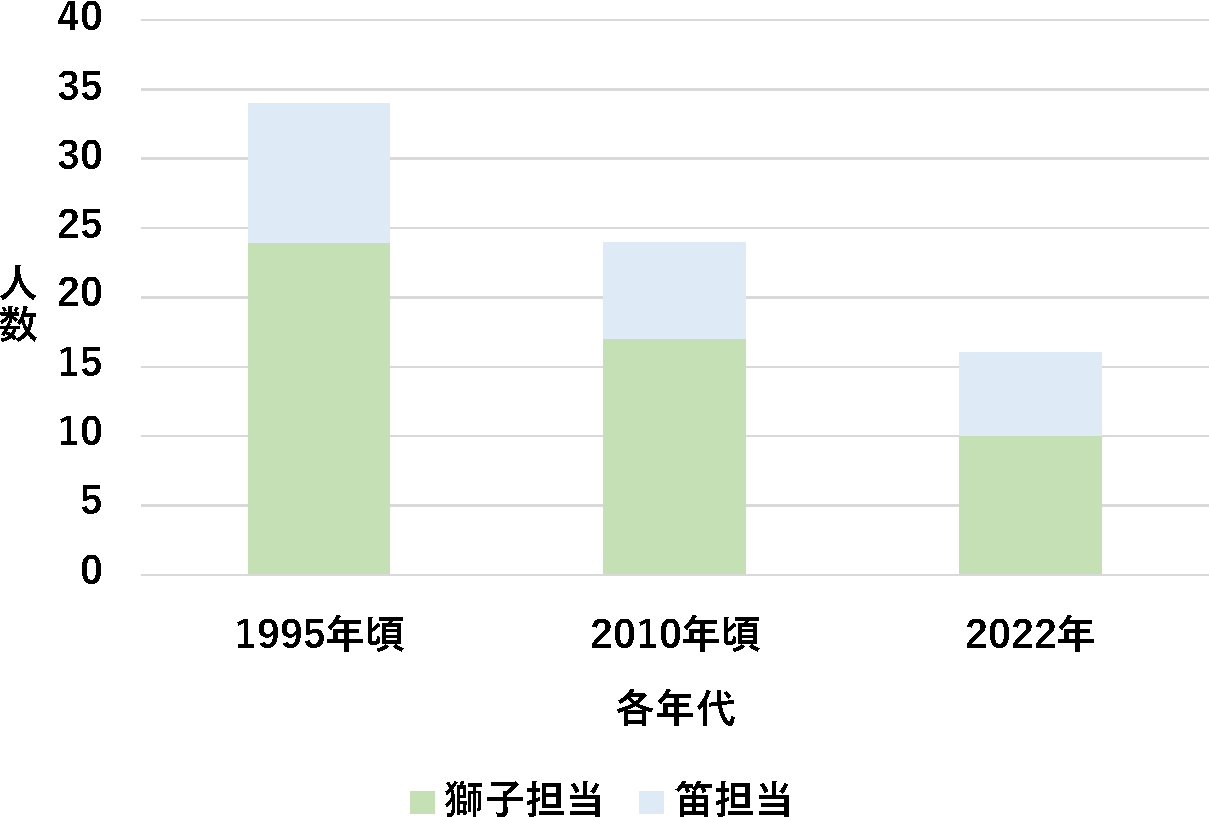
\includegraphics[clip,width=85mm]{figures/hozonkaikazu.pdf}
\end{center}
 \caption{ささら保存会の人数推移}
 \label{fig:図5}
\end{figure}


\subsection{小学生とささら}
地元の下辺見小学校では,児童が女沼のささらを披露する機会がある.児童の中には,4年生から6年生で構成される,ささら代表に参加する児童もいる.

小学校の運動会では全校生徒によるささら発表があるのだが,代表児童が中心となってささらを披露する.その際に,代表児童は,10舞ある女沼のささらの内,
「出羽」「平庭」の2幕を披露する.運動会の他にも地域のお祭りで披露する機会がある.



\subsection{小学生がささらを習得する際の問題点}
ささら代表児童は,小学校の代表としてささらを踊るため,ささらの演技を立派にこなす必要がある.そのため,運動会や祭り前にささら保存会
の方々が,代表児童に数回ささらの指導を行う.

しかし,保存会の方々が代表児童にささらを教える際に問題がある.ささら保存会の人数は図\ref{fig:図5}で示した通り人数が減少しており,舞の指導を行える人
限られてしまっている.以前は約10名で指導を行っていたが,後継者不足と仕事の都合などで,現在では3,4でしか指導を行えない状況である.そのため,代表児童
1人1人に目を向けることが難しくなり,全体に指導がいきわたらない.また,保存会の高齢化の影響で,
小学生の前でささら舞をその場で実演することが難しく,教えられる内容が限られてしまう.

上記の問題を解決するために,本研究ではささら学習教材を開発した.
\newpage
\section{開発した学習教材について}
\subsection{コンセプト}
こんなことができる
ささら学習教材は,個人で女沼のささら舞を学習できるWeb教材である.
ささら代表児童1人1人が本教材で学習することによって,ささら保存会の負担を軽減し,
ささらを踊る上で十分な情報を得ることができる仕様となっている.本教材とささら保存会の数回の指導を
組み合わせることによって,以前より上手に踊れることを想定している.

\subsection{概要}
こんな機能がある
工夫した点は,主に良い例と悪い例の動画や写真を用いて解説し,児童に踊りのポイントを意識させて,理解しやすくした点である.

大まかに,太鼓のたたき方などの「基本」,実際に運動会で踊る「出羽」「平庭」の3つを選択できる構成とした.
この内,基本では,良い例と悪い例の動画と写真を用いて解説し,6つの動作を学習してもらう.
出羽と平庭では,はじめに正面,ななめから撮影した,踊りのポイントごとに番号が出現する踊りの通し動画を視聴してもらい,その出現した番号ごとに
良い例悪い例の動画と写真を用いて解説を行う.1視点のみの通し動画であると,動画の中の3人の動きが重なってしまい,見ずらい箇所がある.
そのため,本教材では2視点の通し動画を提示し,満遍なく3人の動きを視聴できるようにした.出羽は6つ,平庭は4つのポイントを解説する.


\subsection{使い方}
本教材のトップページでは,上段に画面の説明を,中段に「基本」「出羽」「平庭」の3つを選択できるボタンを提示するようにした.学習者
自分の学習したい項目を選択することが可能である.トップページの画面を図\ref{fig:top}に示す.
\vskip\baselineskip
\begin{figure}[h]
\begin{center}
 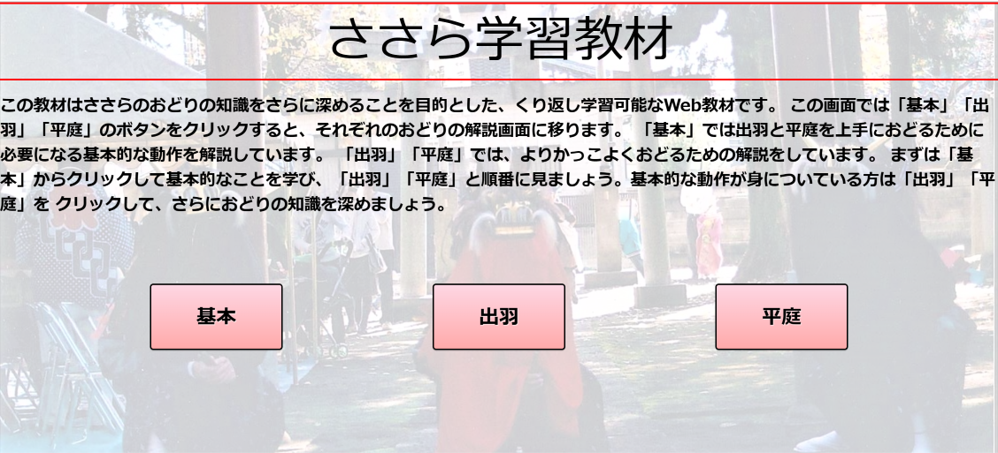
\includegraphics[clip,width=85mm]{figures/top.png}
\end{center}
 \caption{ささら学習教材トップページ}
 \label{fig:top}
\end{figure}

基本では,ささらを上手に踊るために必要な6つの動作を学習してもらう.ここで学習する内容は出羽や平庭にも通じており,主に初級者向けの内容となっている.
基本の画面を図\ref{fig:kihontop}に示す.上段に画面の説明を,中段に6つの動作を選択できるボタンを提示するようにした.内容は左から「道中太鼓」「太鼓のたたき方」
「弓の引き方」「ぶっちじめ」「構え」「首ふり」となっている.
\vskip\baselineskip
\begin{figure}[h]
\begin{center}
  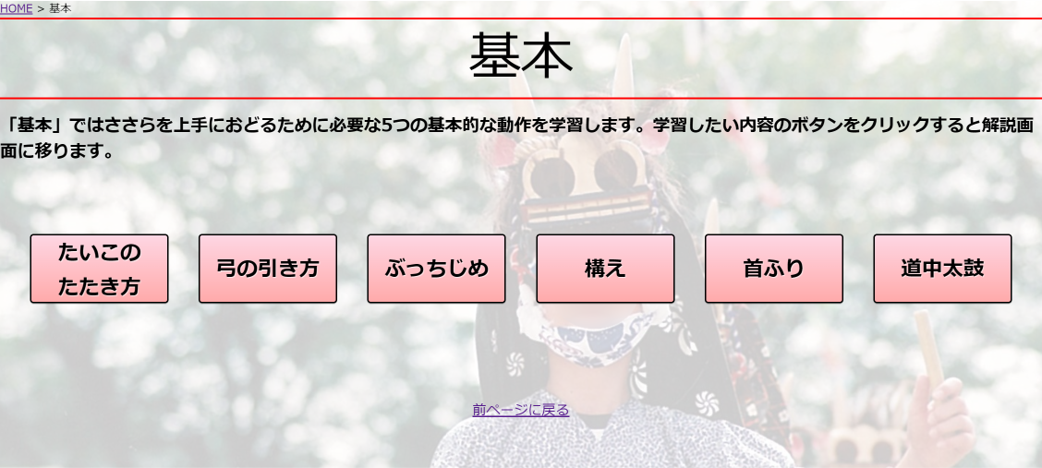
\includegraphics[clip,width=85mm]{figures/kihontop.png}
\end{center}
 \caption{基本画面1}
 \label{fig:kihontop}
\end{figure}
\noindent
例として,太鼓のたたき方を選択した画面を図\ref{fig:kihon2}に示す.
上段に説明文を,中段左に良い例の映像を,中段右に悪い例の映像を,下段に学習者に注目してほしい点を提示している.
\vskip\baselineskip
\begin{figure}[h]
\begin{center}
  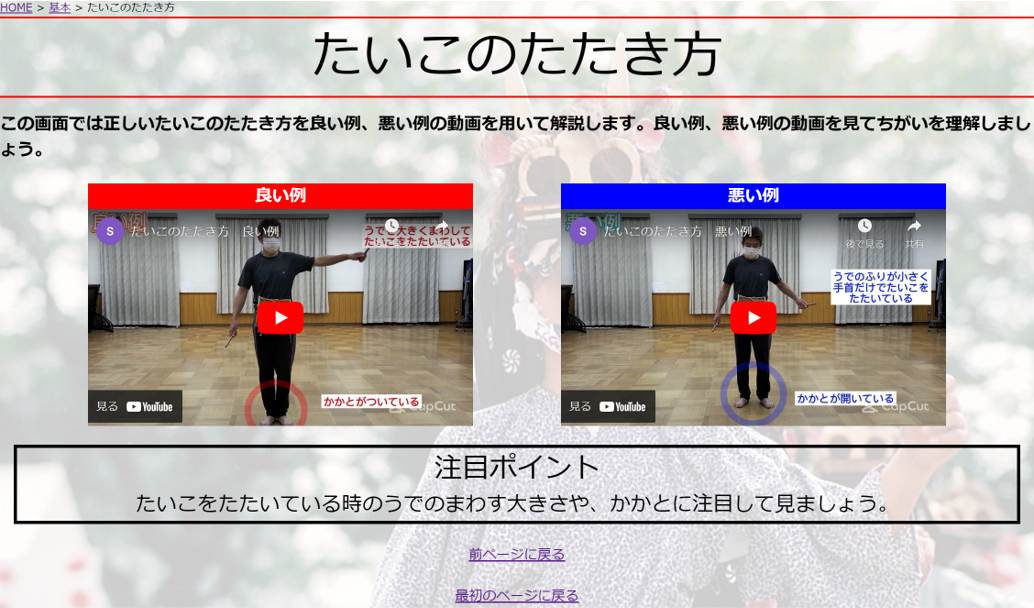
\includegraphics[clip,width=85mm]{figures/kihon2.png}
\end{center}
 \caption{たいこのたたき方の解説画面}
 \label{fig:kihon2}
\end{figure}

出羽では,代表児童が間違えて覚えてしまっている動作を中心に,ささら保存会の方が毎年教えているポイントを学習してもらう.
出羽の画面を図\ref{fig:dewatop}に示す.上段に画面の説明を,中段左に斜めから撮影した通し動画を,中段右に正面から撮影した通し動画を,下段に踊りのポイント
番号を提示している.

\vskip\baselineskip
\begin{figure}[h]
\begin{center}
  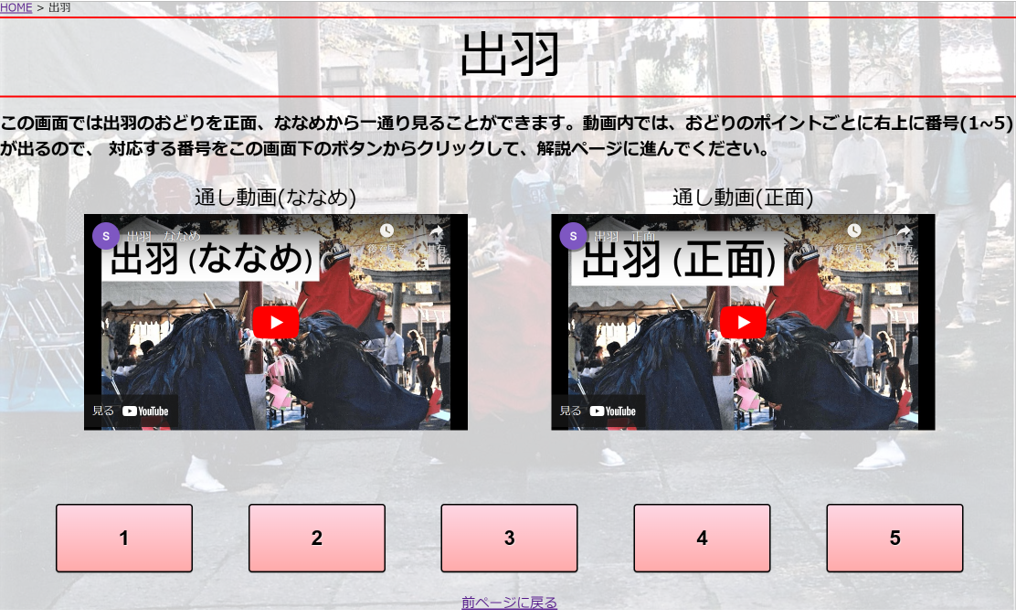
\includegraphics[clip,width=85mm]{figures/dewatop.png}
\end{center}
 \caption{出羽画面}
 \label{fig:dewatop}
\end{figure}
\noindent
ポイント番号については,斜め,正面から撮影した通し動画を視聴すると,図\ref{fig:dewa2}のように,動画内でポイントごとに右上に番号が出現するようになっているため,その対応する
ポイント番号をクリックすると,ポイントの解説ページに遷移する.
\vskip\baselineskip
\begin{figure}[h]
\begin{center}
  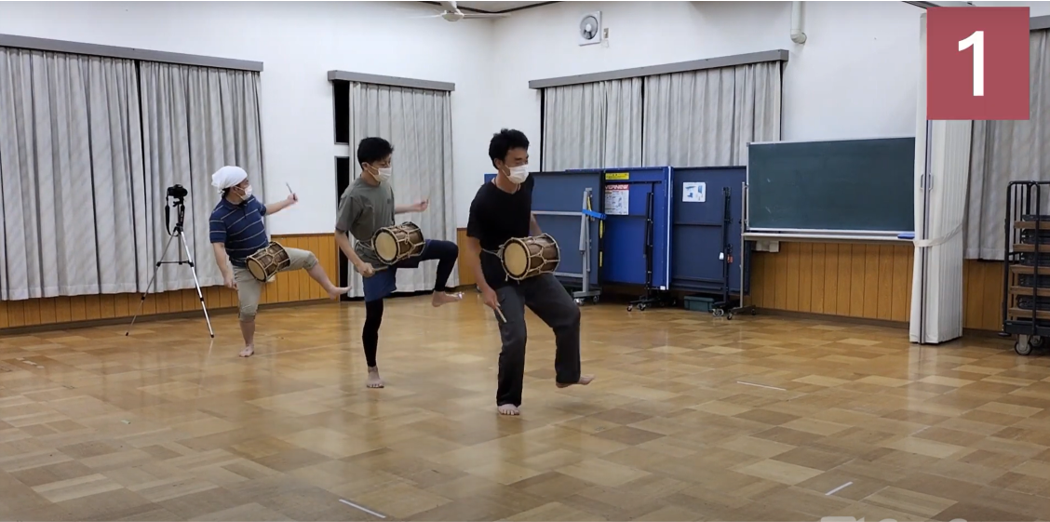
\includegraphics[clip,width=85mm]{figures/dewa2.png}
\end{center}
 \caption{出羽 斜めから撮影した通し動画}
 \label{fig:dewa2}
\end{figure}
\noindent
例として,ポイント番号1を選択した画面を図\ref{fig:dewa3}に示す.基本のたいこのたたき方を選択した画面と構成は同じである.

平庭は出羽と操作方法が同じなため,割愛する.

\vskip\baselineskip
\begin{figure}[h]
\begin{center}
  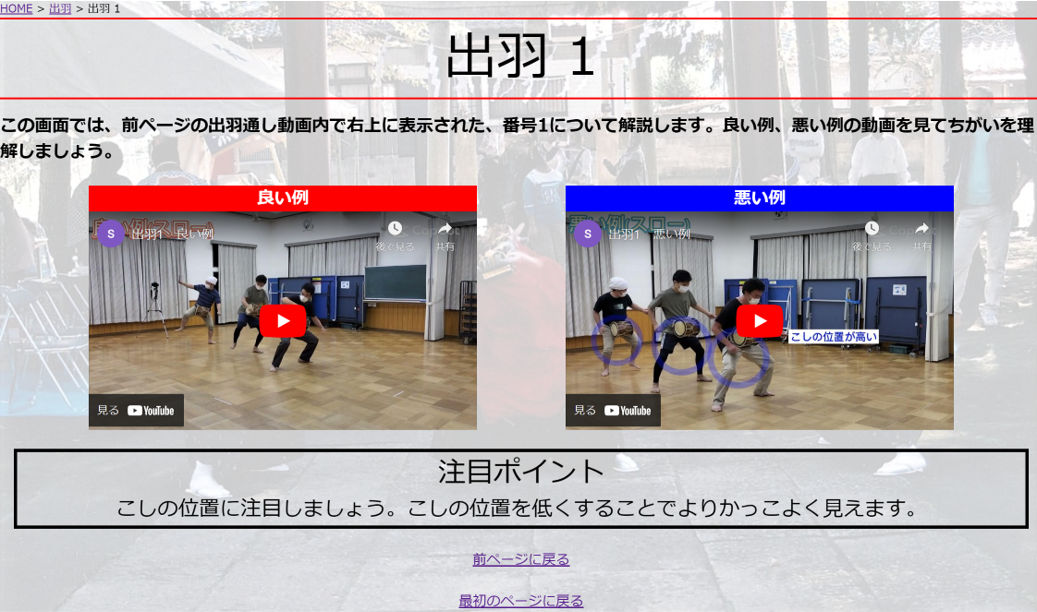
\includegraphics[clip,width=85mm]{figures/dewa3.png}
\end{center}
 \caption{出羽 ポイント番号1の画面}
 \label{fig:dewa3}
\end{figure}
\section{学習教材の評価}
\subsection{アンケート調査}
本教材の有用性を示すために,ささら代表児童にアンケート用紙で調査を行った.対象は,小学6年生5名である.本調査は,ささら保存会の方々の協力の元,祭り前の練習中に
実施した.

アンケートは全9項目あり,大きく分けると,教材の使いやすさ,工夫した点の評価,実用的の3種類について調査した.

回答方法は,「とてもそう思う」「そう思う」「そう思わない」「全くそう思わない」の4つの選択肢から回答してもらい,一週間の回答期間を設けた.
\subsection{アンケート結果}
9項目のアンケ―ト結果を下記に示す.
\vskip\baselineskip
\begin{figure}[h]
\begin{center}
  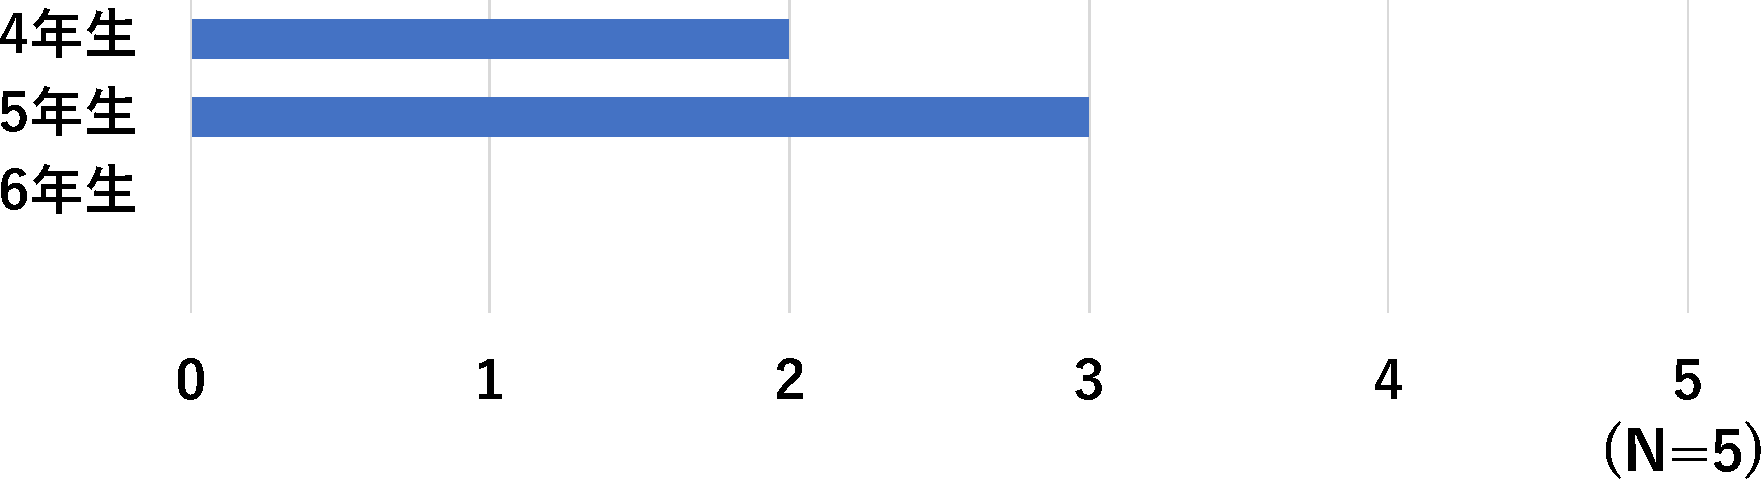
\includegraphics[clip,width=100mm]{figures/anket/an1.pdf}
\end{center}
 \caption{ささら代表児童に何年生の時になりましたか}
 \label{fig:an1}
\end{figure}

\newpage
\subsubsection{教材の使いやすさについての設問}

\vskip\baselineskip
\begin{figure}[h]
\begin{center}
  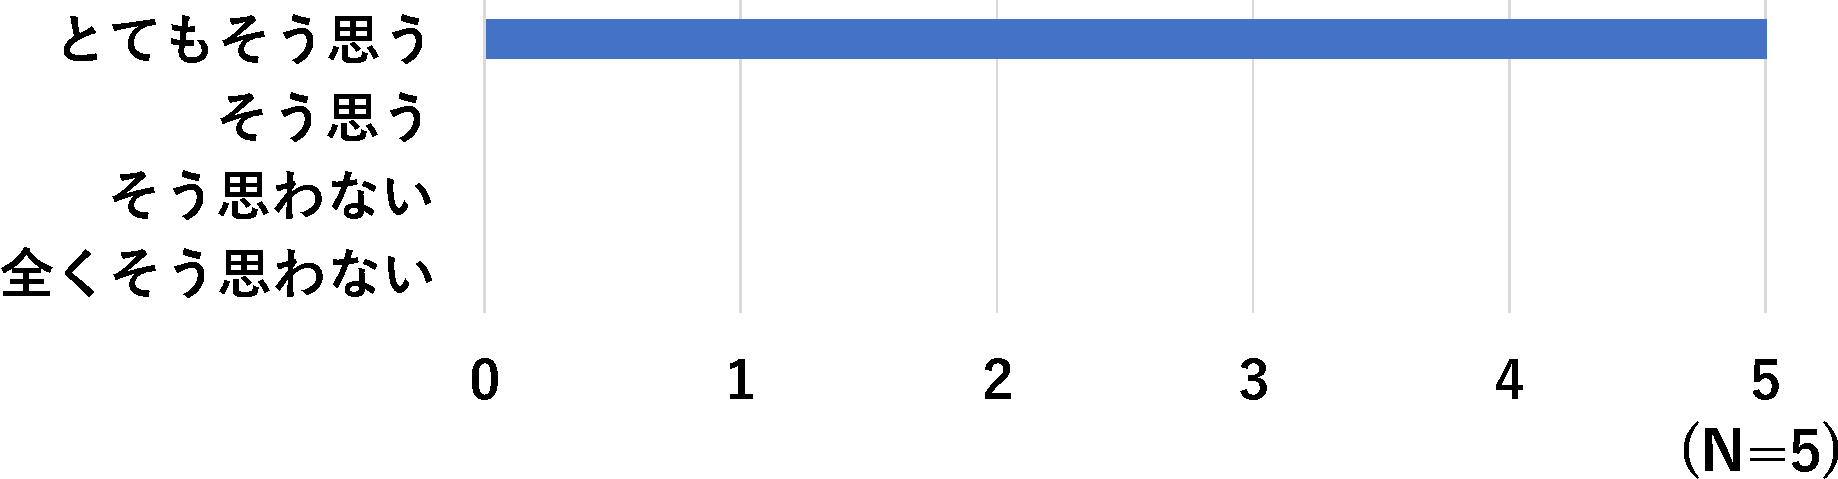
\includegraphics[clip,width=100mm]{figures/anket/an2.pdf}
\end{center}
 \caption{ささら学習教材は使いやすかったですか}
 \label{fig:an1}
\end{figure}

\vskip\baselineskip
\begin{figure}[h]
\begin{center}
  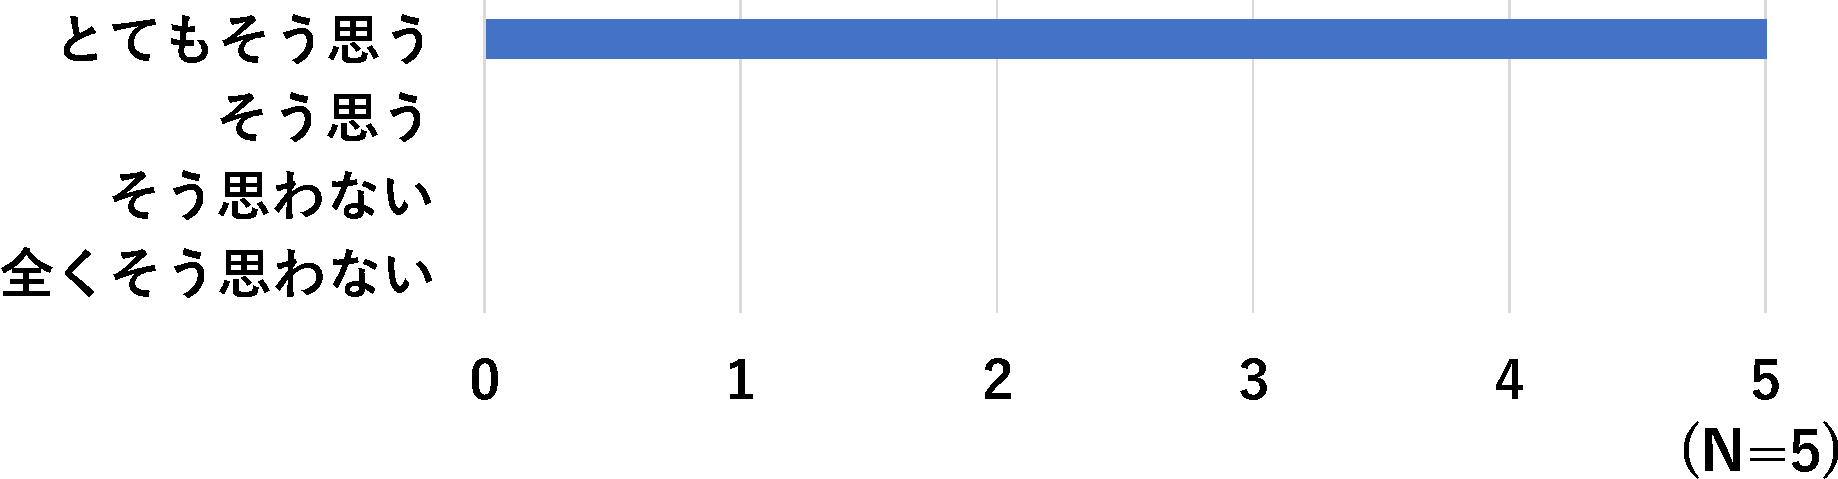
\includegraphics[clip,width=100mm]{figures/anket/an3.pdf}
\end{center}
 \caption{自分の見たいページにたどり着くことができましたか}
 \label{fig:an1}
\end{figure}

\vskip\baselineskip
\begin{figure}[h]
\begin{center}
  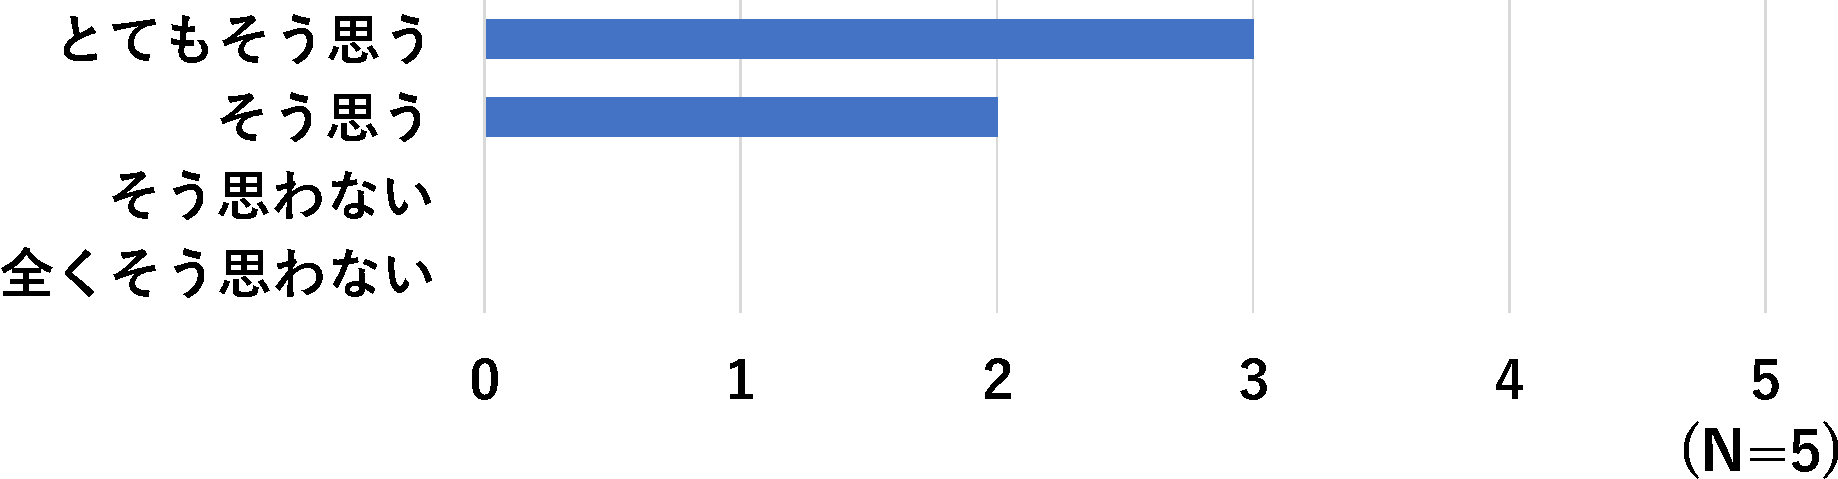
\includegraphics[clip,width=100mm]{figures/anket/an7.pdf}
\end{center}
 \caption{ボタンの大きさや文字の大きさは適切でしたか}
 \label{fig:an1}
\end{figure}

\newpage
\subsubsection{工夫した点の評価についての設問}


\vskip\baselineskip
\begin{figure}[h]
\begin{center}
  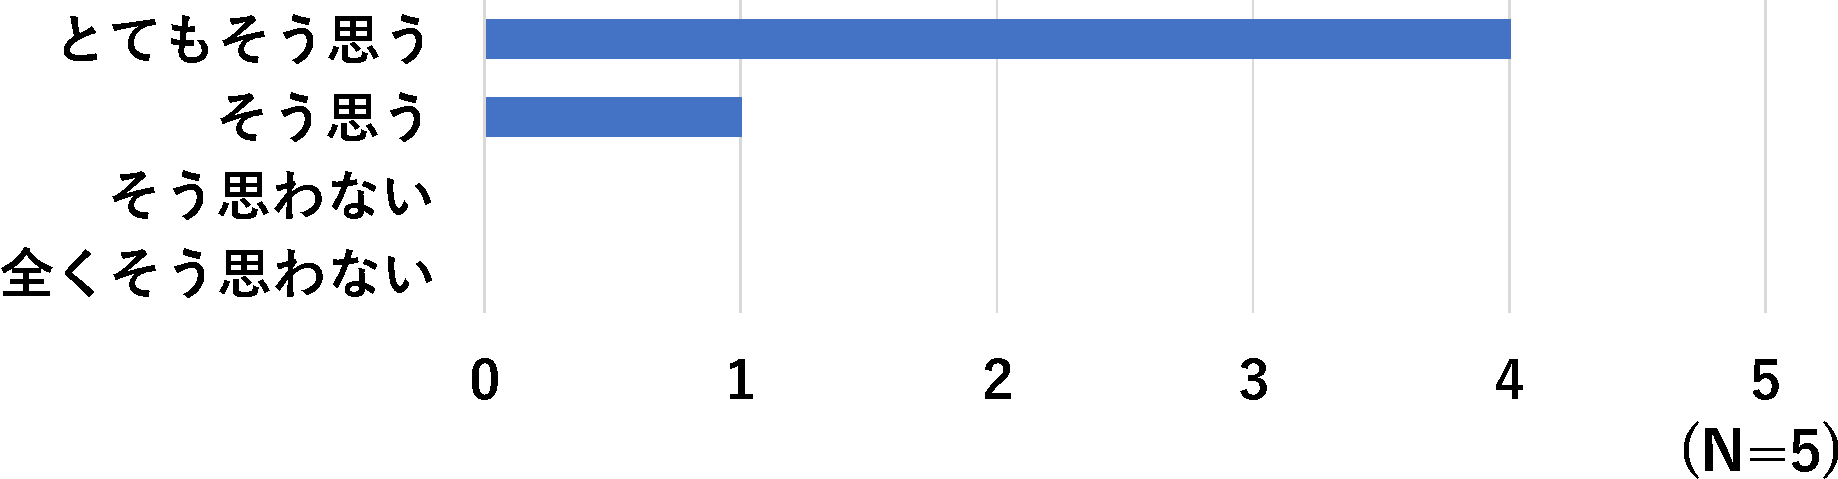
\includegraphics[clip,width=100mm]{figures/anket/an5.pdf}
\end{center}
 \caption{良い例と悪い例の動画や写真を見比べて,自分のまちがいに気づくことができましたか}
 \label{fig:an1}
\end{figure}

\vskip\baselineskip
\begin{figure}[h]
\begin{center}
  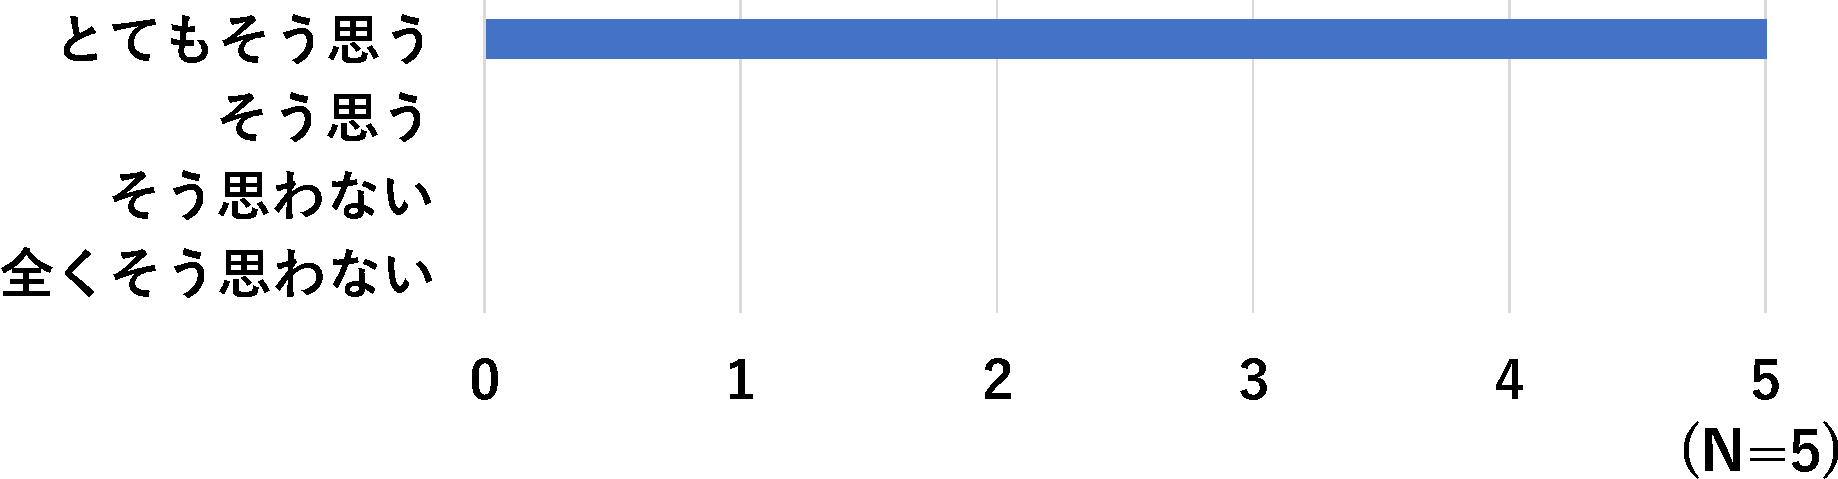
\includegraphics[clip,width=100mm]{figures/anket/an6.pdf}
\end{center}
 \caption{良い例と悪い例を用いて解説しているページで,十分なおどりの情報を得ることができましたか}
 \label{fig:an1}
\end{figure}

\newpage
\subsubsection{実用的についての設問}
\vskip\baselineskip
\begin{figure}[h]
\begin{center}
  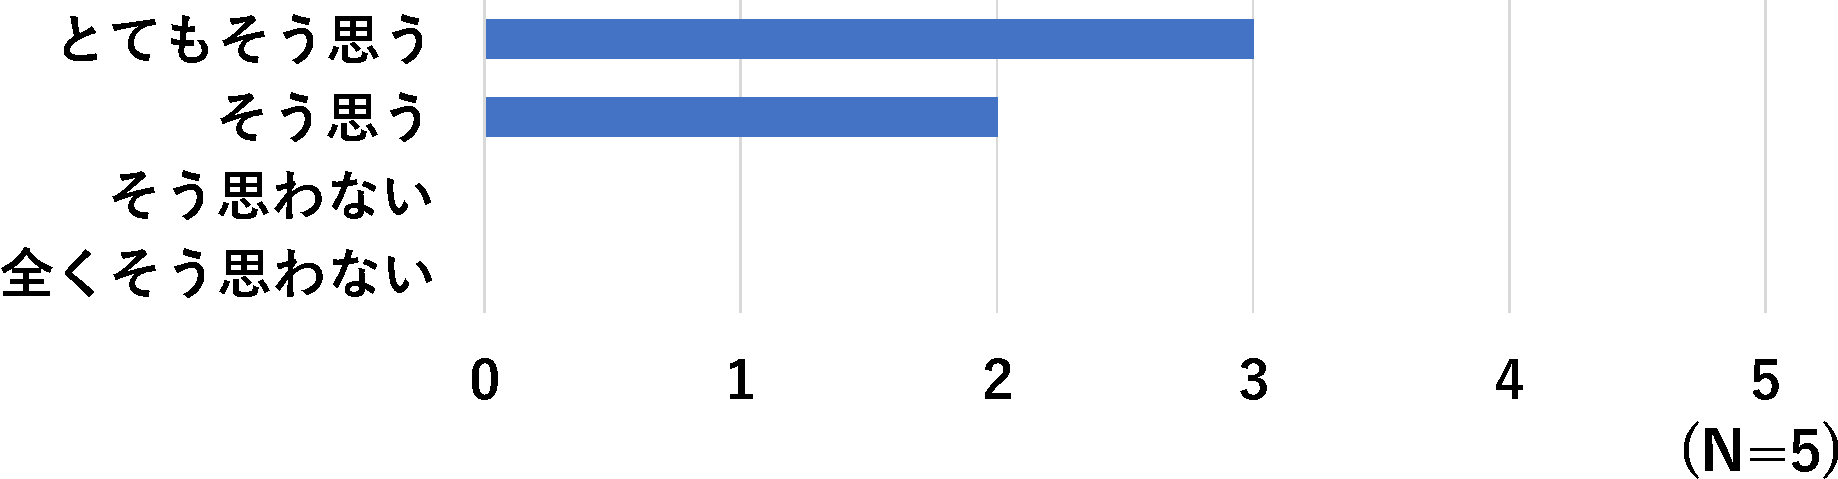
\includegraphics[clip,width=100mm]{figures/anket/an4.pdf}
\end{center}
 \caption{1人でささら学習教材を用いてささらのおどりを学習することができましたか}
 \label{fig:an1}
\end{figure}

\vskip\baselineskip
\begin{figure}[h]
\begin{center}
  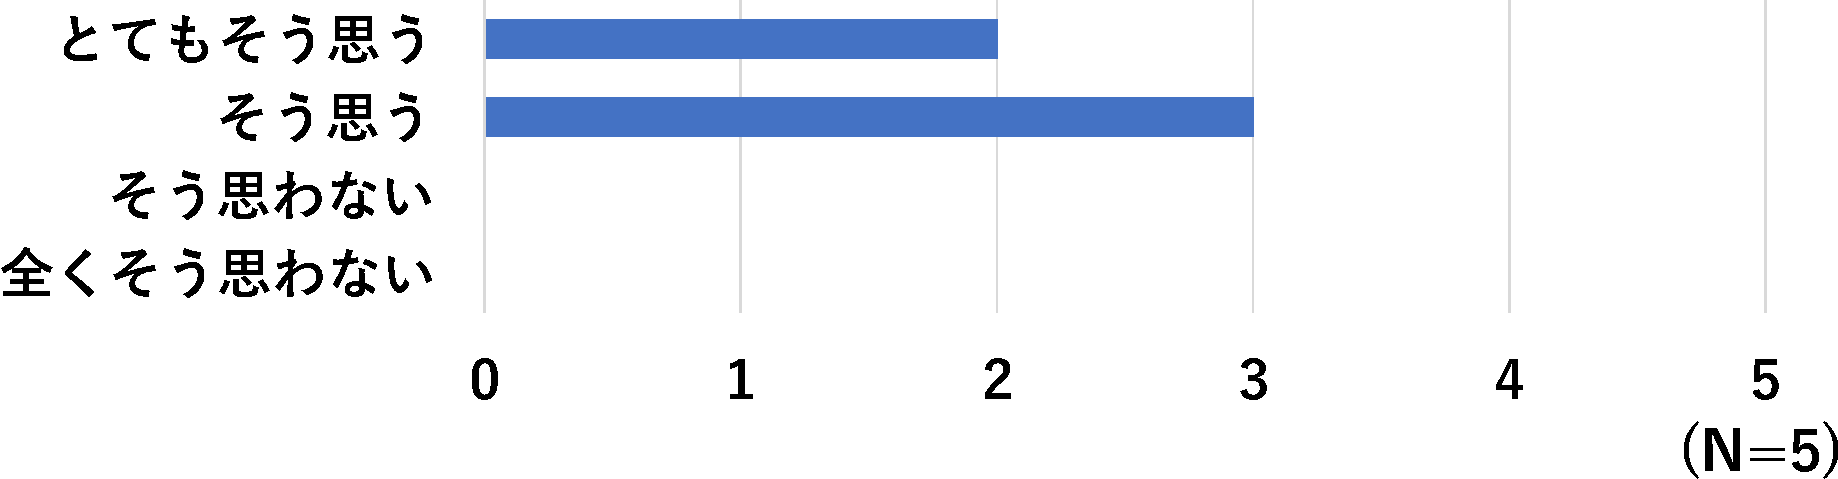
\includegraphics[clip,width=100mm]{figures/anket/an8.pdf}
\end{center}
 \caption{ささら保存会の,年に数回(運動会前や祭りの前)だけでささらを上手におどれると思いますか}
 \label{fig:an1}
\end{figure}

\vskip\baselineskip
\begin{figure}[h]
\begin{center}
  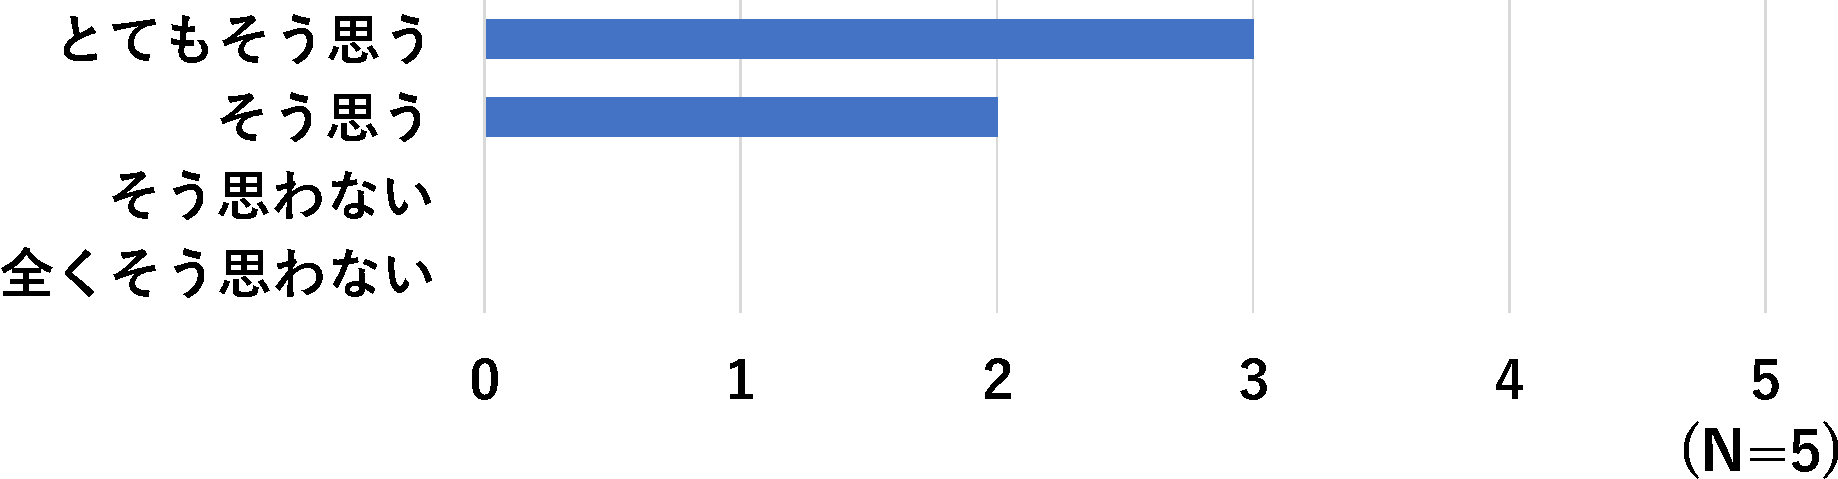
\includegraphics[clip,width=100mm]{figures/anket/an9.pdf}
\end{center}
 \caption{ささら保存会の教えと,ささら学習教材を組み合わせれば今までより上手におどれると思いますか}
 \label{fig:an1}
\end{figure}








\subsection{考察}
アンケート結果より
\section{結言}
\addcontentsline{toc}{section}{参考文献}
\begin{thebibliography}{99}
\bibitem{sa1} 総務省行政評価局: ``伝統工芸の地域資源としての活用に関する実態調査結果報告'', \url{https://www.soumu.go.jp/main_content/000818488.pdf}, 2023/1/1 参照  
\bibitem{sa2} Iwanichi Online 岩手日日新聞社: ``民俗芸能団体運営課題 「後継者不足」最多 北上市連合会 伝承の維持厳しく'', \url{https://www.iwanichi.co.jp/2018/11/05/250225/}, 2023/1/1 参照
\bibitem{sa3} 古河市 生涯学習課: ``女沼のささら(市指定文化財)/古河市公式ホームページ'', \url{https://www.city.ibaraki-koga.lg.jp/soshiki/syogaigakusyu/15/2403.html}, 2022/8/8 参照

\footnote{「太夫獅子」は「前獅子」ともいう}

\end{thebibliography}





\end{document}


